\chapter{Related work} \label{ch:related_work}
In this chapter we present the work related to this study.

\section{Refactoring suggestion tools}
We are novel in the introduction of a fully automated refactoring tool. However, several tools have already been proposed for refactoring suggestion. In this section we discuss these tools. The tools are ordered on basis of the year in which they were proposed.

\subsection{SUPREMO}
A thesis by Golomingi~\cite{koni2001scenario} is the first to explore mapping the relation between clone instances to refactoring methods. The author analyses the refactoring methods described by Martin Fowler \cite{fowler1999refactoring}. Mapping these to relations between clones, this results in Table \ref{tab:relationrefactoring}.

\begin{table}[H]
\centering
\resizebox{\textwidth}{!}{%
\begin{tabular}{lcccccccc}
\toprule
                     & Ancestor   & \begin{tabular}[c]{@{}l@{}}Common\\ Hierarchy\end{tabular} & \begin{tabular}[c]{@{}l@{}}First\\ Cousin\end{tabular} & \begin{tabular}[c]{@{}l@{}}Same\\ Method\end{tabular} & Sibling    & \begin{tabular}[c]{@{}l@{}}Single\\ Class\end{tabular} & Superclass & Unrelated \\ \midrule
Extract Method       & \checkmark & \checkmark                                                 & \checkmark                                             & \checkmark                                            & \checkmark & \checkmark                                             &            &           \\
Insert Method Call   &            &                                                            &                                                        & \checkmark                                            &            & \checkmark                                             &            &           \\
Insert Super Call    &            &                                                            &                                                        &                                                       &            &                                                        & \checkmark &           \\
Parameterization     & \checkmark & \checkmark                                                 & \checkmark                                             & \checkmark                                            & \checkmark & \checkmark                                             & \checkmark &           \\
Pull Up Method       & \checkmark & \checkmark                                                 & \checkmark                                             &                                                       & \checkmark &                                                        & \checkmark &           \\
Form Template Method & \checkmark & \checkmark                                                 & \checkmark                                             & \checkmark                                            & \checkmark & \checkmark                                             & \checkmark &           \\
Push Down Method     &            &                                                            &                                                        &                                                       &            &                                                        & \checkmark &           \\
Extract Superclass   &            & \checkmark                                                 & \checkmark                                             &                                                       & \checkmark &                                                        &            &           \\ \bottomrule
\end{tabular}%
}
\caption{Mapping clone relations to refactoring techniques \cite{koni2001scenario}}
\label{tab:relationrefactoring}
\end{table}

The author then proposes a tool named ``SUPREMO''. This tool determines the relations between clone instances, computes the impact of the clones and proposes refactorings. Their tool features visualizations to show how clones are related in the inheritance structure. This tool is written for the Smalltalk programming language. The authors verify their approach by presenting several cases in which their tool analyses source code and outputs a refactoring suggestion.

\subsection{Aries}
A study by Higo et al.~\cite{higo2004aries, higo2008metric} looks into to what extent clones can be refactored. They show code examples and to what entent they can be cloned. For instance, they look into what parts of a clone can be extracted to a new method. They define that partially cloned blocks obstruct method extraction. They propose t make the clone smaller to find a part of the clone that can be refactored. This is similar to our ``partial block'' category of Section~\ref{sec:refactorabilitysetup} and our discussion in Section~\ref{sec:partialblockdiscussion}.

Higo et al. also look into the amount of variability that can be allowed between clone fragments. Figure~\ref{fig:higomerge} shows an example of merging two code fragments from this study. In this figure, the clone spans a part of a different block so it cannot be refactored. However, they propose to ommit both ``else if'' lines from the merged fragment so that it can be refactored (in our study we would have flagged these clones as ``partial block'' and thus unsuitable for refactoring). They also allow variability in literals and variables and replace them with method parameters.

\begin{figure}[H]
  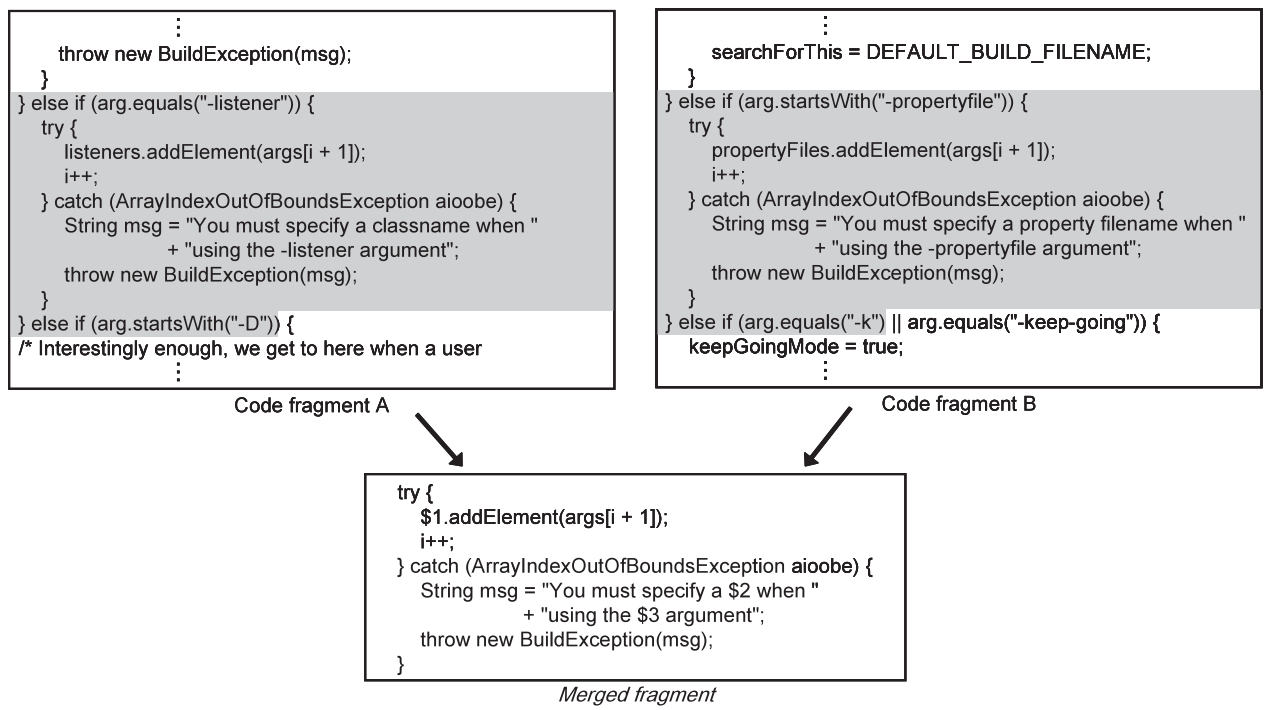
\includegraphics[width=1\textwidth]{img/higo}
  \caption{Example of merging two code fragments from Higo et al.~\cite{higo2008metric}.}
  \label{fig:higomerge}
\end{figure}

Higo et al. propose a tool named Aries~\cite{higo2004aries, higo2008metric} that focuses on the detection of refactorable clones. They focus entirely on whether a clone \textbf{can} be refactored and not whether it \textbf{should} be refactored. This tool only proposes refactoring opportunities and does not provide help in the process of applying the refactoring.

\subsection{Duplicated Code Refactoring Advisor (DCRA)}
Fontana et al.~\cite{fontana2012duplicated, fontana2015duplicated} combine the research by Golomingi~\cite{koni2001scenario} with clone types \cite{roy2007survey}. They use a large corpus~\cite{tempero2010qualitas} on which they perform statistical analysis of clone relations together with clone types. Table \ref{tab:dcra-relation} displays the result of this analysis. We added percentages and ordering to this table for easier comparison with the results of our studies (see \ref{sec:relationresults}).

\begin{table}[H]
\centering
\begin{tabular}{@{}lllll@{}}
\toprule
                         & Type 1 & Percentage & Type 3 & Percentage \\ \midrule
Same Class               & 5,645  & 32.1\%     & 51,308 & 28.7\%     \\
Same External Superclass & 4,384  & 25.0\%     & 66,391 & 37.1\%     \\
Unrelated Class          & 2,758  & 15.7\%     & 35,035 & 19.6\%     \\
Sibling Class            & 2,721  & 15.5\%     & 13,868 & 7.8\%      \\
Common Hierarchy Class   & 970    & 5.5\%      & 3,152  & 1.8\%      \\
Same Method              & 569    & 3.2\%      & 4,901  & 2.7\%      \\
First Cousin Class       & 416    & 2.4\%      & 2,980  & 1.7\%      \\
Superclass               & 91     & 0.5\%      & 981    & 0.5\%      \\
Ancestor Class           & 13     & 0.1\%      & 281    & 0.2\%      \\ \bottomrule
\end{tabular}
\caption{Clone relation analysis by Fontana et al. \cite{fontana2012duplicated} for type 1 and 3 clones measured over the Qualitas Corpus \cite{tempero2010qualitas}.}
\label{tab:dcra-relation}
\end{table}

Fontana et al.~\cite{fontana2012duplicated, fontana2015duplicated} propose DCRA, a tool to suggest refactorings for the clones found by the NiCAD tool \cite{roy2008nicad, cordy2011nicad}. DCRA suggests refactorings to clones found in Java projects based on the mapping between relation and refactoring techniques shown in Table~\ref{tab:relationrefactoring}.

\subsection{Refactoring Technique for Large Groups of Software Clones}
A thesis by AlWaqfi~\cite{alwaqfi2017refactoring} propose a method for assessing refactorability of clone classes (whereas the previous tools only focus on clone pairs). The author surveys a set of clone detection tools \cite{kamiya2002ccfinder, baxter1999clonedr, jiang2007deckard, cordy2011nicad} and uses a publicly available dataset \cite{tsantalis2015assessing} to measure the amount of clones found by these tools. The resulting data shows that significant portions of source code of the measured systems are cloned. The data also shows that there are large differences between different tools in the amount of clones found. The author also measures of how many clone instances clone classes consist. According to these experiments, about 68\% of clone classes consist of 2 clone instances, 13\% have 3 clone instances, 7\% have 4 clone instances and about 12\% is even larger.

The authors perform a lot of statistical comparisons between clone detection tools. The part most relevant to our study is their measurements regarding refactorability. They find that about 29-54\% of clones are refactorable in the set of projects they inspect (Table 6.13 of \cite{alwaqfi2017refactoring}). To determine whether a clone is refactorable, the author states a list of eight preconditions for a cloned fragment to be refactorable. These preconditions are similar to the categories we identified in Section~\ref{sec:refactorabilitysetup}.

\subsection{Pattern‐based clone Refactoring Inspection (PRI)}
A study by Chen et al.~\ref{chen2018clone} addresses the problem that developers cannot easily determine which clones can be refactored or how they should be maintained scattered
throughout a large code base in evolving systems. They propose PRI, a technique for managing clone refactorings for clones with a Sibling relation. PRI is a plugin for the Eclipse IDE that shows which refactoring techniques can be used to refactor clones. Because it is integrated in the Eclipse IDE, the refactorings can be executed largely automatically, as this IDE has a large set of tools for performing such transformations.

PRI traces clones through revisions of a software project. This makes this tool able to find incompletely refactored clones. PRI produces false positives in that several groups are incorrectly classified since the clone detector suffers the inaccuracy in finding semantically equivalent behaviors between clones.
